% Test report: power-loss-tolerant supercapacitor logger on the MSP-EXP430FR5994
% Build:  pdflatex lab_report ; bibtex lab_report ; pdflatex lab_report ; pdflatex lab_report
% The earlier paper-style version is kept in paper.tex.
\documentclass[11pt,a4paper]{article}

\usepackage[T1]{fontenc}
\usepackage[utf8]{inputenc}
\usepackage{lmodern}
\usepackage[margin=2.3cm, headheight=14pt]{geometry}
\usepackage{cite}
\usepackage{amsmath,amssymb}
\usepackage{graphicx}
\usepackage{booktabs}
\usepackage{tabularx}
\usepackage{longtable}
\usepackage{float}
\usepackage{array}
\usepackage{siunitx}
\usepackage{enumitem}
\usepackage[table]{xcolor}
\usepackage{url}
\usepackage{fancyhdr}
\usepackage{titlesec}
\usepackage{tikz}
\usetikzlibrary{positioning,arrows.meta,fit,calc,backgrounds,shapes.geometric}
\usepackage{pgfplots}
\usepgfplotslibrary{groupplots}
\pgfplotsset{compat=1.18}
\usepackage[hidelinks]{hyperref}

\sisetup{detect-all, per-mode=symbol}
\newcommand{\uA}{\,\si{\micro\ampere}}
\newcommand{\mA}{\,\si{\milli\ampere}}
\newcommand{\uC}{\,\si{\micro\coulomb}}
\newcommand{\code}[1]{\texttt{#1}}
\newcolumntype{L}{>{\raggedright\arraybackslash}X}
\setlist{itemsep=1pt,topsep=3pt}
\setlength{\parindent}{0pt}
\setlength{\parskip}{5pt}

\newcommand{\docid}{TR-01}
\newcommand{\docrev}{1.1}

\pagestyle{fancy}
\fancyhf{}
\lhead{\small Supercapacitor logger -- test report}
\rhead{\small \docid{} Rev.~\docrev}
\cfoot{\small \thepage}
\renewcommand{\headrulewidth}{0.4pt}

\titleformat{\section}{\large\bfseries}{\thesection}{0.6em}{}
\titleformat{\subsection}{\normalsize\bfseries}{\thesubsection}{0.6em}{}

% ---- verdict tags ----
\newcommand{\pass}{\textbf{\textcolor{green!45!black}{PASS}}}
\newcommand{\fail}{\textbf{\textcolor{red!70!black}{FAIL}}}
\newcommand{\recorded}{\textbf{\textcolor{blue!60!black}{RECORDED}}}
\newcommand{\pending}{\textbf{\textcolor{orange!80!black}{PENDING}}}
\newcommand{\partly}{\textbf{\textcolor{orange!80!black}{PARTIAL}}}

% ---- test-case header block ----
% \testcase{ID}{Title}{label}{Objective}{Build}{Power and jumpers}{Acceptance criterion}
\newcommand{\testcase}[7]{%
  \subsection{#1 -- #2}\label{#3}
  \noindent\begin{tabularx}{\textwidth}{@{}>{\raggedright\arraybackslash\bfseries}p{3.6cm}L@{}}
  \toprule
  Objective & #4 \\
  Firmware build & #5 \\
  Power and jumpers & #6 \\
  Acceptance criterion & #7 \\
  \bottomrule
  \end{tabularx}\par\medskip}

\begin{document}

% =====================================================================
\begin{titlepage}
\centering
\vspace*{1.5cm}
{\large Pontifical Catholic University of Rio de Janeiro (PUC-Rio)\par}
\vspace{2.2cm}
{\LARGE\bfseries Test Report\par}
\vspace{0.4cm}
{\Large Power-Loss-Tolerant, Supercapacitor-Powered\\ Data Logger on the MSP-EXP430FR5994\par}
\vspace{1.6cm}
{\large Jo\~{a}o Gabriel Peixoto\par}
{\normalsize joaogdrumond@aluno.puc-rio.br\par}
\vspace{1.6cm}
\begin{tabular}{@{}ll@{}}
\toprule
Document & \docid{}, revision \docrev \\
Device under test & MSP-EXP430FR5994 LaunchPad, onboard 0.22\,F supercapacitor \\
Firmware & Logger application with Layer 1--3 drivers (\code{driver\_development}) \\
Toolchain & Code Composer Studio 12.5, TI MSP430 CGT 21.6.1 \\
Test dates & 21--22 November 2026 \\
\bottomrule
\end{tabular}
\vfill
\begin{minipage}{0.86\textwidth}\small
\textbf{AI-assistance disclosure.} This work was carried out with the assistance of Claude (Anthropic), an AI assistant. Under my direction it wrote the firmware, analysed the measurement data, and drafted this report and its figures. I ran all hardware tests and I am responsible for the content.
\end{minipage}
\vspace{1cm}
\end{titlepage}

\section*{Revision history}
\begin{tabularx}{\textwidth}{@{}llL@{}}
\toprule
Rev. & Date & Changes \\
\midrule
1.0 & 21 Nov 2026 & First issue as a test report. Covers tests T1--T11; T12 (full supercapacitor drain) is pending. Supersedes the paper-style write-up kept in \code{paper.tex}. \\
1.1 & 22 Nov 2026 & T12 results added (overnight run, pass with notes). Running-time statements revised: the drain falls with the voltage, so constant-drain estimates are pessimistic. Issue I-6 extended with the T12 deep-sleep drain. \\
\bottomrule
\end{tabularx}

\tableofcontents
\newpage

% =====================================================================
\section{Purpose and scope}

This report records the tests I ran on a data logger built for the MSP-EXP430FR5994 LaunchPad. The logger runs only from the board's 0.22\,F supercapacitor. Every 2\,s it measures its own supply voltage (VCC) and die temperature and stores them in FRAM. Its firmware is a three-layer driver stack written from the register level, plus the logger application.

The tests answer four questions:
\begin{enumerate}
  \item Does the saved state survive power loss at any moment, without corruption? (T3, T4)
  \item Does the supply-aware power policy enter and leave deep sleep correctly, with the clock continuous? (T5)
  \item How much current does the logger draw, and where does it go? (T6--T9)
  \item How long does it actually run from the supercapacitor, and do the long history log and the clock recovery work on hardware? (T2, T10--T12)
\end{enumerate}

\textbf{In scope:} the drivers, the logger application, the command console and their behaviour on one LaunchPad.
\textbf{Out of scope:} energy harvesting, other boards, and temperature extremes. All tests ran at room temperature on one board.

Section~\ref{sec:summary} gives the results at a glance. Section~\ref{sec:dut} describes the device under test, Section~\ref{sec:setup} the setup and measurement method, and Section~\ref{sec:tests} each test in detail. Open issues are logged in Section~\ref{sec:issues}.

% =====================================================================
\section{Background}

Batteryless and energy-harvesting sensors run from small stores such as capacitors, and their supply can collapse at any moment~\cite{hester2017future,lucia2017snapl}. Their firmware has to keep its state across power losses, avoid spending energy it does not have, and recover by itself. FRAM makes the first part practical: it is non-volatile, byte-addressable and cheap to write, so state can be saved often~\cite{jayakumar2014quickrecall}.

Research on \emph{intermittent computing} has explored several ways to do this. Mementos~\cite{ransford2011mementos} inserts trigger points at compile time and checkpoints volatile state to flash when the supply voltage is low. Hibernus~\cite{balsamo2015hibernus} watches the supply and takes one snapshot as late as possible, when failure is imminent. QuickRecall~\cite{jayakumar2014quickrecall} uses FRAM as unified memory, so that only registers need saving. DINO~\cite{lucia2015dino} shows that checkpointing volatile state alone can leave non-volatile data inconsistent, and proposes task boundaries with data versioning. Capybara~\cite{colin2018capybara} reconfigures the energy store itself to match each task.

This project works at the application level instead. The state that matters (counters and a sample log) is small and explicit, so it is saved as a whole after every change. Its consistency comes from an atomic two-copy commit in the spirit of shadow paging~\cite{lorie1977physical}, with a CRC~\cite{koopman2004crc} to detect torn or corrupted copies. Like Hibernus, the logger reacts to its supply voltage, but it does so by entering the device's LPMx.5 shutdown mode~\cite{ti_slau367} and waiting for the supply to recover.

% =====================================================================
\section{Summary of results}
\label{sec:summary}

\begin{table}[H]
\centering\small
\caption{Test summary}
\label{tab:summary}
\begin{tabularx}{\textwidth}{@{}l>{\raggedright\arraybackslash}p{4.6cm}Ll@{}}
\toprule
ID & Test & Result & Verdict \\
\midrule
T1 & Build verification & All 12 configurations build without warnings & \pass \\
T2 & History log unit test (PC) & 9/9 scenarios correct, including torn records and wrap-around & \pass \\
T3 & Random power cuts & 36 cuts: 0 restore failures, 0 inconsistent copies, 0 saves lost & \pass \\
T4 & Fault injection in a save & 9/9 steps restored exactly the predicted copy & \pass \\
T5 & Deep-sleep cycle on USB & 9/9 wakes on the RTC minute, clock continuous, 3/3 resumes & \pass \\
T6 & Logger energy profile & 3.2--4.4\uA{} average; floor varies by $\sim$1\uA{} between sessions & \recorded \\
T7 & Deep-sleep energy & 2.10--2.25\uA{} floor, $\sim$1\uC{} per minute wake & \recorded \\
T8 & Status-LED A/B, one capture & 7.41 $\rightarrow$ 4.10\uA{} (-45\,\%), floor unchanged & \pass \\
T9 & Console energy, one capture & Idle console: no measurable cost; streaming +5.5\uC{} per line & \pass \\
T10 & Supercapacitor run, 82\,min & 5.4\uA{} total drain; history and clock recovery correct over 9 boots & \pass \\
T11 & Supercapacitor run, 12\,min & 4.8\uA{} total drain, consistent with T10; issue I-1 found & \pass \\
T12 & Overnight supercapacitor run & 10.8\,h logging from 2.78\,V; drain fell from 4.3 to 2.7\uA; deep sleep at 2.199\,V with 109 minute wakes; brown-out not reached & \pass{} (notes) \\
\bottomrule
\end{tabularx}
\end{table}

In short, the store survived every power cut and every injected fault, and the power policy behaved as designed. Measured in Free Run, the logger draws 3.2--4.4\uA. On the supercapacitor, where the capacitor's own leakage also counts, the drain is 4.8--5.4\uA{} near 2.8--2.96\,V (T10, T11) and falls to 2.7\uA{} near 2.2\,V (T12). The overnight run logged for 10.8\,h from a 2.78\,V charge, 67\,\% longer than a constant-drain estimate, then held in deep sleep with minute wakes as designed. It passed with notes: it did not start from a full charge and did not reach brown-out. A code review, T11 and T12 found six open issues, none of which affected the results above (Section~\ref{sec:issues}).

% =====================================================================
\section{Device under test}
\label{sec:dut}

\subsection{Hardware}

The MSP430FR5994 has 256\,KB of FRAM, 8\,KB of SRAM, a 12-bit ADC with an internal reference and temperature sensor, a calendar RTC and four eUSCI\_A UARTs~\cite{ti_slase54}. Each device also carries factory calibration data in its TLV (Tag-Length-Value) table, a protected memory area at 0x1A00. The drivers use it to correct the internal reference voltages, the ADC gain and offset, and the temperature sensor, which TI measured at 30 and 85\,\textdegree C~\cite{ti_slau367}. On the LaunchPad, jumper J8 connects the 0.22\,F supercapacitor. In the \emph{Charge} position, USB powers the board and charges the capacitor. In the \emph{Use} position, the capacitor is tied directly to the 3.3\,V rail, so VCC is the capacitor voltage~\cite{ti_slau678}. The onboard eZ-FET debugger provides programming, a USB backchannel UART on eUSCI\_A0, and EnergyTrace energy measurement~\cite{ti_slaa603}. The J101 jumper block connects the eZ-FET to the target.

\subsection{Firmware architecture}

Fig.~\ref{fig:arch} shows the three driver layers and the application. \emph{Layer~1} brings up the board in the order the hardware requires: it holds the watchdog, latches the reset cause, puts every pin into a low-power state, configures the crystal pins, and only then releases the I/O lock (LOCKLPM5). Port interrupt flags are cleared only after a cold start, because after an LPMx.5 wake they hold the wake event~\cite{ti_slau367}. The clock driver runs the DCO at 8\,MHz and starts the 32.768\,kHz crystal with a timeout and a fall-back to the internal VLO. \emph{Layer~2} adds the voltage reference, the ADC (VCC through the internal \(\tfrac{1}{2}\)\,AVCC divider, die temperature through the calibrated sensor), RTC, timers, CRC and the checkpoint store. \emph{Layer~3} adds an interrupt-driven UART driver and a command console. Appendix~\ref{app:modules} describes each module.

\begin{figure}[tbp]
\centering
\resizebox{\textwidth}{!}{%
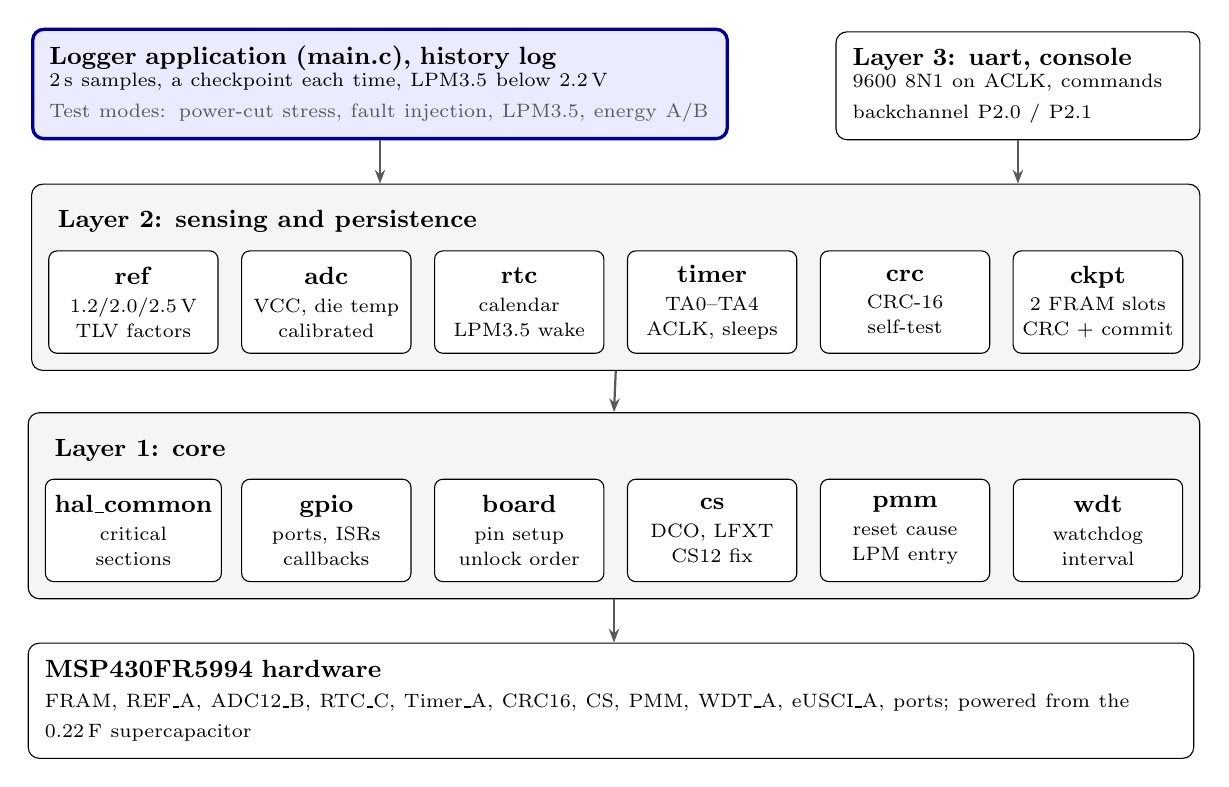
\begin{tikzpicture}[
  font=\small,
  drv/.style={draw, rounded corners=3pt, minimum width=2.15cm, minimum height=1.3cm, align=center, fill=white},
  lay/.style={draw, rounded corners=4pt, fill=gray!8, inner sep=6pt},
  arr/.style={-{Stealth[length=5pt]}, thick, gray!70!black}
]
  \node[drv] (ref)   at (0,0)     {\textbf{ref}\\[-1pt]\scriptsize 1.2/2.0/2.5\,V\\[-2pt]\scriptsize TLV factors};
  \node[drv] (adc)   at (2.45,0)  {\textbf{adc}\\[-1pt]\scriptsize VCC, die temp\\[-2pt]\scriptsize calibrated};
  \node[drv] (rtc)   at (4.9,0)   {\textbf{rtc}\\[-1pt]\scriptsize calendar\\[-2pt]\scriptsize LPM3.5 wake};
  \node[drv] (tim)   at (7.35,0)  {\textbf{timer}\\[-1pt]\scriptsize TA0--TA4\\[-2pt]\scriptsize ACLK, sleeps};
  \node[drv] (crc)   at (9.8,0)   {\textbf{crc}\\[-1pt]\scriptsize CRC-16\\[-2pt]\scriptsize self-test};
  \node[drv] (ckpt)  at (12.25,0) {\textbf{ckpt}\\[-1pt]\scriptsize 2 FRAM slots\\[-2pt]\scriptsize CRC + commit};
  \node[anchor=south west] (l2t) at ($(ref.north west)+(0,0.1)$) {\textbf{Layer 2: sensing and persistence}};
  \node[drv] (hal)   at (0,-2.9)     {\textbf{hal\_common}\\[-1pt]\scriptsize critical\\[-2pt]\scriptsize sections};
  \node[drv] (gpio)  at (2.45,-2.9)  {\textbf{gpio}\\[-1pt]\scriptsize ports, ISRs\\[-2pt]\scriptsize callbacks};
  \node[drv] (board) at (4.9,-2.9)   {\textbf{board}\\[-1pt]\scriptsize pin setup\\[-2pt]\scriptsize unlock order};
  \node[drv] (cs)    at (7.35,-2.9)  {\textbf{cs}\\[-1pt]\scriptsize DCO, LFXT\\[-2pt]\scriptsize CS12 fix};
  \node[drv] (pmm)   at (9.8,-2.9)   {\textbf{pmm}\\[-1pt]\scriptsize reset cause\\[-2pt]\scriptsize LPM entry};
  \node[drv] (wdt)   at (12.25,-2.9) {\textbf{wdt}\\[-1pt]\scriptsize watchdog\\[-2pt]\scriptsize interval};
  \node[anchor=south west] (l1t) at ($(hal.north west)+(0,0.1)$) {\textbf{Layer 1: core}};
  \begin{scope}[on background layer]
    \node[lay, fit=(ref)(ckpt)(l2t)] (L2) {};
    \node[lay, fit=(hal)(wdt)(l1t)] (L1) {};
  \end{scope}
  \node[draw=blue!60!black, very thick, fill=blue!8, rounded corners=4pt, align=left, text width=8.4cm, inner sep=6pt,
        anchor=south west] (app) at ($(L2.north west)+(0,0.55)$)
        {\textbf{Logger application (main.c), history log}\\ \scriptsize 2\,s samples, a checkpoint each time, LPM3.5 below 2.2\,V\\ \scriptsize\color{gray!70!black} Test modes: power-cut stress, fault injection, LPM3.5, energy A/B};
  \node[draw, rounded corners=4pt, align=left, text width=4.2cm, inner sep=6pt, anchor=south east, fill=white]
        (l3) at ($(L2.north east)+(0,0.55)$)
        {\textbf{Layer 3: uart, console}\\ \scriptsize 9600 8N1 on ACLK, commands\\ \scriptsize backchannel P2.0 / P2.1};
  \node[draw, rounded corners=4pt, align=left, anchor=north west, inner sep=6pt, text width=14.38cm]
        (hw) at ($(L1.south west)+(0,-0.55)$)
        {\textbf{MSP430FR5994 hardware}\\ \scriptsize FRAM, REF\_A, ADC12\_B, RTC\_C, Timer\_A, CRC16, CS, PMM, WDT\_A, eUSCI\_A, ports; powered from the 0.22\,F supercapacitor};
  \draw[arr] (app.south) -- (app.south |- L2.north);
  \draw[arr] (l3.south) -- (l3.south |- L2.north);
  \draw[arr] (L2.south) -- (L1.north);
  \draw[arr] (L1.south) -- (L1.south |- hw.north);
\end{tikzpicture}}
\caption{Firmware architecture. The application uses drivers from all layers and never touches peripheral registers directly, so every test mode runs on the same drivers as the logger.}
\label{fig:arch}
\end{figure}

Table~\ref{tab:errata} lists the errata and datasheet constraints the drivers handle. The most consequential are PMM31/PMM32: entering LPM2--4 with FRAM powered can fail, so every low-power entry runs from RAM and powers FRAM down first~\cite{ti_slaz681}.

\begin{table}[H]
\centering\small
\caption{Errata and constraints handled in the drivers~\cite{ti_slaz681,ti_slase54}}
\label{tab:errata}
\begin{tabularx}{\textwidth}{@{}lL@{}}
\toprule
Item & Handling \\
\midrule
PMM31/32 & LPM2--4 entry from RAM with FRAM powered down; ADC used in active mode only \\
CS12 & Clock dividers $\geq$\,/4 around a DCO change, $\sim$10\,\textmu s settle \\
ADC42 & BUSY checked before every conversion \\
ADC71 & ENC and SC set in separate writes \\
ADC67 & API to override the TLV temperature calibration \\
USCI42 & UART end of transmission from UCBUSY, not UCTXCPTIFG \\
FRAM & One wait state above 8\,MHz (NWAITS) \\
REF/AVCC & 1.2\,V reference below 2.4\,V VCC; each reference needs its minimum AVCC \\
LPMx.5 & RTC and ports reconfigured before LOCKLPM5 is cleared; wake flags kept \\
\bottomrule
\end{tabularx}
\end{table}

\subsection{Checkpoint store}
\label{sec:ckpt}

The application state (boot, power-loss and deep-sleep counters, sample count, minimum VCC, and a 16-entry log of time, VCC and temperature) lives in RAM and is saved to FRAM after every change. The store keeps two slots in persistent FRAM. Each holds a magic word, length, sequence number, CRC-16/CCITT and payload. A save always writes the slot that does \emph{not} hold the newest valid copy, in this order:
\begin{enumerate}
  \item mark the slot invalid;
  \item write payload, length and sequence number;
  \item write the CRC over length, sequence and payload;
  \item mark the slot valid (the commit point).
\end{enumerate}
Restore returns the valid slot with the highest sequence number. A power cut before step~4 leaves the previous copy as the newest valid one; a cut after it leaves the new copy. A torn or bit-flipped slot fails its CRC and is ignored. The CRC is computed by the hardware CRC16 module and checked at boot against a software reference.

\subsection{History log and clock recovery}
\label{sec:hist}

The checkpoint holds only the newest 16 samples (32\,s), which is too short for a discharge test. A separate ring of 1600 records (22.4\,KB of FRAM) stores one record every 60 samples (2\,min) while logging, plus one at each boot, deep-sleep entry, minute wake, resume and clock change. Each record is committed like a checkpoint slot: it is invalidated first and its one-byte valid mark is written last. A 16-bit sequence number orders the records, and a persistent hint lets a boot find the newest record without scanning the whole ring. The hint is checked at boot and repaired if a cut left it one record behind.

The RTC driver keeps the time across LPMx.5 wakes and across resets that leave the RTC running with a valid date. A brown-out clears the RTC. After one, the firmware restarts the clock one second after the newest logged time, so timestamps never run backwards. The clock is then behind by the length of the outage, and the boot record flags it as restored.

\subsection{Supply-aware power policy}

Fig.~\ref{fig:fsm} shows the policy. While VCC is at least 2.2\,V, the RTC wakes the CPU from LPM3 every 2\,s to take a sample, save a checkpoint and service a 16\,s watchdog. A green LED flashes for 2\,ms once per pass through the 16-entry log. Below 2.2\,V the logger saves, shuts the console down and enters LPM3.5, where only the RTC runs~\cite{ti_slau367}. An RTC minute event wakes it. That wake is a reset, so it passes through boot and restore, measures VCC, and goes back to LPM3.5 unless VCC has recovered to 2.6\,V. The 400\,mV hysteresis keeps the logger from oscillating at the threshold.

\begin{figure}[tbp]
\centering
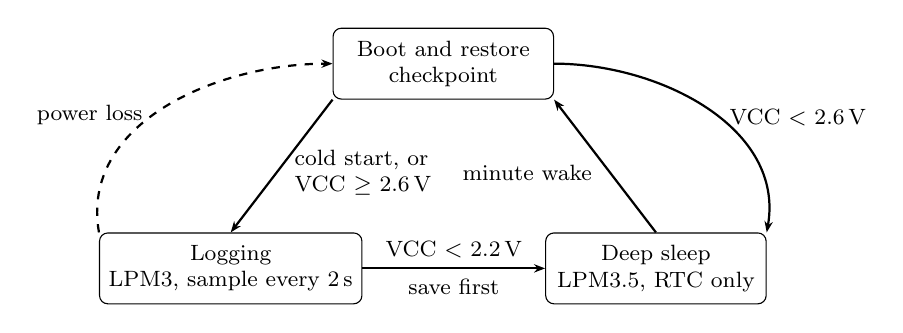
\begin{tikzpicture}[font=\footnotesize,
  st/.style={draw, rounded corners=3pt, align=center, minimum height=9mm, minimum width=2.8cm, fill=white},
  arr/.style={-{Stealth[length=4pt]}, thick}]
  \node[st] (boot) at (0,0)      {Boot and restore\\checkpoint};
  \node[st] (log)  at (-2.7,-2.6) {Logging\\LPM3, sample every 2\,s};
  \node[st] (deep) at (2.7,-2.6)  {Deep sleep\\LPM3.5, RTC only};
  \draw[arr] (boot.south west) -- node[right, pos=0.55, xshift=1mm, align=left] {cold start, or\\VCC $\geq$ 2.6\,V} (log.north);
  \draw[arr] (deep.north) -- node[left, pos=0.45, xshift=-1mm] {minute wake} (boot.south east);
  \draw[arr] (log.east) -- node[above] {VCC $<$ 2.2\,V} node[below] {save first} (deep.west);
  \draw[arr] (boot.east) to[out=0, in=80] node[right, pos=0.55] {VCC $<$ 2.6\,V} (deep.north east);
  \draw[arr, dashed] (log.north west) to[out=100, in=180] node[left, pos=0.45] {power loss} (boot.west);
\end{tikzpicture}
\caption{Supply-aware power policy. Cold starts, power losses (brown-out resets) and minute wakes from LPM3.5 all pass through checkpoint restore.}
\label{fig:fsm}
\end{figure}

\subsection{Command console}

The console runs on the backchannel UART at 9600\,baud, clocked from the 32\,kHz crystal with the divider settings from the user's guide~\cite{ti_slau367} (UCBRx\,=\,3, UCBRSx\,=\,0x92), so the CPU stays in LPM3 while bytes move and wakes for one short interrupt per byte. It has seven commands:
\begin{itemize}
  \item \code{help} -- list the commands;
  \item \code{status} -- time and its source, boot reason, counters, VCC, temperature;
  \item \code{log} -- the 16-sample log as CSV;
  \item \code{hist [n]} -- the history log as CSV, or its newest $n$ records;
  \item \code{time [YYYY-MM-DD hh:mm:ss]} -- show or set the clock;
  \item \code{stream} -- print each sample as it is taken;
  \item \code{erase yes} -- clear the state and the history.
\end{itemize}
Timestamps are seconds since 2026-01-01, computed from the calendar date with Hinnant's civil-date algorithms~\cite{hinnant_date}; the conversion was checked on the PC against a reference calendar for 49\,000 consecutive days.

\subsection{Build configurations}

Test behaviour is selected with compile-time switches (Table~\ref{tab:switches}). The release build has all of them at 0. Only one may be 1 at a time; the build rejects any other combination.

\begin{table}[H]
\centering\small
\caption{Test switches}
\label{tab:switches}
\begin{tabularx}{\textwidth}{@{}llL@{}}
\toprule
Switch & File & Effect when 1 \\
\midrule
\code{CKPT\_STRESS\_TEST} & \code{main.c} & Continuous saves for unplug testing (T3) \\
\code{CKPT\_FAULT\_TEST} & \code{drivers/ckpt.h} & Cut points in \code{ckpt\_save}, fault sequence (T4) \\
\code{LPM35\_TEST} & \code{main.c} & Scheduled LPM3.5 episodes on USB power (T5, T7) \\
\code{LED\_AB\_TEST} & \code{main.c} & LED every sample for 75 samples, then every 16th (T8) \\
\code{CONSOLE\_E10\_TEST} & \code{main.c} & Console off / idle / streaming in one capture (T9) \\
\bottomrule
\end{tabularx}
\end{table}

% =====================================================================
\section{Test setup and method}
\label{sec:setup}

\subsection{Equipment}

\begin{itemize}
  \item MSP-EXP430FR5994 LaunchPad (one unit), with its eZ-FET debugger and 0.22\,F supercapacitor.
  \item PC with Code Composer Studio 12.5 and the TI MSP430 code generation tools 21.6.1; EnergyTrace through the eZ-FET.
  \item Serial terminal on the ``MSP Application UART1'' port at 9600\,baud, 8N1.
  \item Visual Studio 2022 C compiler for the PC unit test (T2).
\end{itemize}

\subsection{Board configurations}

\begin{table}[H]
\centering\small
\caption{Board configurations used in the tests}
\label{tab:configs}
\begin{tabularx}{\textwidth}{@{}lLl@{}}
\toprule
Name & Jumpers and supply & Used in \\
\midrule
USB & USB connected, J8 in Charge (or removed), all J101 jumpers fitted & T1, T3--T5 \\
Energy & USB connected, J8 removed so capacitor charging and leakage stay out of the measurement; EnergyTrace in Free Run & T6--T9 \\
Supercap & J8 in Use, USB unplugged after charging; console read after reconnecting & T10--T12 \\
\bottomrule
\end{tabularx}
\end{table}

\subsection{Robustness tests}

The robustness tests (T3--T5) use build modes that record their results in persistent FRAM, so the results survive the resets the tests provoke. I read them after each test by connecting the debugger with ``load symbols only'', which does not reflash the board or clear FRAM.

\subsection{Energy measurements}
\label{sec:method}

EnergyTrace exports cumulative energy in 0.1\,\textmu J steps at about 1\,kHz. Currents are derived from energy differences over 20--250\,ms bins, and averages are taken over complete 2\,s sample periods, measured from one sample's spike to the next. Each capture lasts 300\,s in Free Run.

\textbf{Same-capture comparisons.} The absolute floor that EnergyTrace reports shifts by up to about 1\uA{} from one session to the next (T6). Charges of individual events, such as one LED flash, stay consistent. I therefore compare firmware variants \emph{inside one capture}: a test switch changes the firmware's behaviour after a fixed number of samples, so both variants share the same calibration (T8, T9). Absolute floors are quoted as ranges.

\textbf{Supercapacitor drain.} On the supercapacitor, the current follows from the voltage slope: $I = C\,dV/dt$ with $C = 0.22$\,F. This includes the capacitor's own leakage and everything else on its side of the board, so it is the number that sets the real running time. I fit straight lines to the 2-minute VCC records of the history log.

% =====================================================================
\section{Test cases}
\label{sec:tests}

% ---------------------------------------------------------------------
\testcase{T1}{Build verification}{t:build}
  {Confirm that every driver and every test configuration builds cleanly.}
  {Release and each test switch alone, at -Ooff and -O2.}
  {Not applicable.}
  {No errors and no warnings in any configuration; RAM and FRAM within limits.}

\textbf{Procedure.} The project was built with its own flags, MPU enabled,
\begin{center}\code{-vmspx -{}-data\_model=restricted -{}-use\_hw\_mpy=F5}\end{center}
in 12 configurations: the release build and the five test switches, each at -Ooff and -O2. A preprocessor check in \code{main.c} stops the build with an error if more than one test switch is 1.

\textbf{Results.} All 12 configurations built without errors or warnings. The release build uses 1.4\,KB of the 4\,KB general-purpose RAM (with a 512-byte stack) and 26\,KB of the 48\,KB lower FRAM region, most of it the 22.4\,KB history ring.

\textbf{Verdict:} \pass

% ---------------------------------------------------------------------
\testcase{T2}{History log unit test on a PC}{t:hist}
  {Check the history log's recovery logic against every power-cut case, before running it on the board.}
  {\code{app/history.c} compiled for the PC with \code{HIST\_HOST\_TEST}; plain arrays stand in for FRAM.}
  {Not applicable.}
  {All scenarios return the expected record count and newest sequence, with every record intact and in order.}

\textbf{Procedure.} A test program fills the ring and simulates reboots by calling \code{hist\_init()} again. Power cuts are simulated by editing the ring and the hint directly. After each scenario it checks the record count, the newest sequence number, that sequence numbers are consecutive, and that every payload is intact.

\begin{table}[H]
\centering\small
\begin{tabularx}{\textwidth}{@{}clL@{}}
\toprule
\# & Scenario & Expected \\
\midrule
1 & Empty ring & Count 0, no newest record \\
2 & 10 records, reboot, 5 more & 15 records in order \\
3 & 5000 records (ring wraps 3 times), reboot & 1600 newest records in order \\
4 & Cut after invalidating the next slot & Torn slot ignored; next record overwrites it \\
5 & Cut between commit and hint update & Hint repaired at boot; no record lost \\
6 & Garbage hint & Full scan finds the newest record \\
7 & Sequence number wraps past 65\,535 & Order kept across the wrap \\
8 & Clear, reboot & Ring empty; restarts at slot 0 with sequence 1 \\
9 & Partly filled ring with a torn next slot & 3 records, torn slot ignored \\
\bottomrule
\end{tabularx}
\end{table}

\textbf{Results.} All nine scenarios passed (``all history tests passed''). The same module then ran on hardware in T10 and T11.

\textbf{Verdict:} \pass

% ---------------------------------------------------------------------
\testcase{T3}{Random power cuts}{t:cuts}
  {Show that the checkpoint store never loses or mixes state when power is cut at random.}
  {\code{CKPT\_STRESS\_TEST = 1}: saves in a tight loop; every field of a copy is derived from one counter, so a mixed copy is detectable.}
  {USB configuration; power cut by unplugging USB.}
  {0 restore failures, 0 inconsistent copies, and at most 1 save lost per cut (the one in progress).}

\textbf{Procedure.}
\begin{enumerate}
  \item Flash the stress build and let it run.
  \item Unplug USB at a random moment, wait a few seconds, plug it back in. Repeat.
  \item After each run, read the result counters in FRAM with the debugger (symbols only).
\end{enumerate}
At each boot the firmware restores the newest copy, checks that its fields agree with each other, and compares it with the last save it recorded before the cut.

\textbf{Results.}
\begin{table}[H]
\centering\small
\begin{tabular}{@{}lccccc@{}}
\toprule
Run & Cuts & Restore failures & Inconsistent copies & Max.\ saves lost & Last saved vs.\ counter \\
\midrule
1 & 10 & 0 & 0 & 0 & 110464 vs 110465 \\
2 & 26 & 0 & 0 & 0 & 264023 vs 264024 \\
\bottomrule
\end{tabular}
\end{table}
The last saved value is one behind the RAM counter because the debugger halt landed inside an unfinished save; restore correctly returned the previous complete copy.

\textbf{Verdict:} \pass{} -- 36 cuts, no failures.

% ---------------------------------------------------------------------
\testcase{T4}{Fault injection in a save}{t:fault}
  {Exercise a power cut at every step of a save, which random cuts cannot target, plus FRAM corruption.}
  {\code{CKPT\_FAULT\_TEST = 1}: \code{ckpt\_save()} has six cut points that trigger a software brown-out reset at an exact step; steps 7--9 corrupt FRAM directly.}
  {USB configuration.}
  {Each step restores exactly the copy the design predicts (table below).}

\textbf{Procedure.} Flash the build and let it run. It walks through the nine steps by itself, resetting the device at each cut point, and records which steps behaved as predicted. Read the result in FRAM with the debugger.

\begin{table}[H]
\centering\small
\begin{tabularx}{\textwidth}{@{}lLl@{}}
\toprule
Step & Fault & Expected outcome \\
\midrule
1 & Reset after the slot is marked invalid & Old copy restored \\
2 & Reset with half the payload written & Old copy restored \\
3 & Reset after the payload, before length and sequence & Old copy restored \\
4 & Reset after length and sequence, before the CRC & Old copy restored \\
5 & Reset after the CRC, before the commit & Old copy restored \\
6 & Reset just after the commit & New copy restored \\
7 & One payload bit flipped in the newest slot & Falls back to the older copy \\
8 & One header bit flipped in the remaining slot & Restore reports failure \\
9 & Save after both copies are lost & New copy restored \\
\bottomrule
\end{tabularx}
\end{table}

\textbf{Results.} \code{passed} = 0x03FE (steps 1--9), \code{failed} = 0, \code{restarts} = 0. The final counter was 5, exactly as predicted (2 $\rightarrow$ 3 at step 6 $\rightarrow$ 4 saved then corrupted $\rightarrow$ 5).

\textbf{Verdict:} \pass{} -- 9/9.

% ---------------------------------------------------------------------
\testcase{T5}{Deep-sleep cycle on USB}{t:lpm35}
  {Check that the logger enters LPM3.5, wakes on each RTC minute, stays asleep while VCC is low, and resumes with the clock continuous.}
  {\code{LPM35\_TEST = 1}: after 5 samples the low threshold is forced above VCC; the first two minute wakes stay asleep and the third applies the real 2.6\,V check, which passes on USB.}
  {USB configuration.}
  {Every wake is an LPMx.5 wake on a minute rollover, 60\,s apart; logging resumes on the third wake; no faults recorded.}

\textbf{Procedure.} Flash the build and leave it for about 10 minutes. Each wake records its RTC time, gap since the last wake, reset code and a fault mask in FRAM. Read them with the debugger.

\textbf{Results.}
\begin{table}[H]
\centering\small
\begin{tabular}{@{}ccccc@{}}
\toprule
Episode & Asleep at (s) & Wakes (s) & First gap (s) & Resumed at (s) \\
\midrule
1 & 3 & 60, 120, 180 & 57 & 180 \\
2 & 187 & 240, 300, 360 & 53 & 360 \\
3 & 367 & 420, 480, 540 & 53 & 540 \\
\bottomrule
\end{tabular}
\end{table}
All nine wakes had reset code 8 (LPMx.5 wake) and fault mask 0. The first gap of each episode is shorter than 60\,s because the logger fell asleep part-way through a minute and the RTC wakes on the rollover.

\textbf{Verdict:} \pass{} -- 9/9 wakes, 3/3 resumes.

% ---------------------------------------------------------------------
\testcase{T6}{Logger energy profile}{t:energy}
  {Measure the logger's average current and sleep floor, and the effect of the firmware optimizations.}
  {Release build, before and after two optimizations: status LED only every 16th sample, and 8-conversion temperature averaging.}
  {Energy configuration; EnergyTrace in Free Run, 300\,s per capture.}
  {Characterization; no pass/fail limit.}

\textbf{Procedure.} Capture 300\,s of the logger before the optimizations, then again after them, and compute the floor and the average over complete sample periods.

\textbf{Results.}
\begin{table}[H]
\centering\small
\begin{tabular}{@{}lccc@{}}
\toprule
Build & Average & Floor & Charge per sample \\
\midrule
LED on every sample & 7.86\uA & 2.62\uA & $\sim$10.4\uC \\
LED every 16th, temperature averaged & 3.21\uA & 1.35\uA & -- \\
\bottomrule
\end{tabular}
\end{table}

The two captures disagree on the floor by 1.27\uA, although nothing in the sleep path changed between the builds. The difference is constant over the whole sleep period. T8 settles the question: when both behaviours run in one capture, the floor stays the same to within 0.013\uA. So the floor difference is a property of the EnergyTrace session, not of the firmware. From here on, firmware variants are compared within one capture, and absolute floors are quoted as ranges (Section~\ref{sec:method}).

\textbf{Verdict:} \recorded{} -- 3.2--4.4\uA{} for the final firmware across sessions (T6, T8, T9).

% ---------------------------------------------------------------------
\testcase{T7}{Deep-sleep energy}{t:lpm35e}
  {Measure the LPM3.5 floor and the cost of a minute wake.}
  {\code{LPM35\_TEST = 1} (as T5), which flashes the LEDs at each wake so wakes are visible.}
  {Energy configuration; Free Run, 300\,s.}
  {Characterization; no pass/fail limit.}

\textbf{Results.} The floor was 2.10--2.25\uA{} across six sleep stretches (Fig.~\ref{fig:traces}b). A minute wake cost about 640\uC, of which about 638\uC{} were the test build's two 100\,ms LED flashes. Without them, a wake costs about 1\uC, an estimate at the resolution of the data, or about 0.02\uA{} averaged over a minute. The datasheet LPM3.5 current is about 0.5\uA~\cite{ti_slase54}; the difference is open issue I-6.

\textbf{Verdict:} \recorded.

\begin{figure}[tbp]
\centering
\begin{tikzpicture}
\begin{groupplot}[group style={group size=1 by 2, vertical sep=13mm},
  width=0.95\textwidth, height=4cm, ymode=log, ymin=1, ymax=5000,
  ytick={1,10,100,1000}, yticklabels={1\,\textmu A,10\,\textmu A,100\,\textmu A,1\,mA},
  tick label style={font=\footnotesize}, label style={font=\footnotesize}, title style={font=\footnotesize, yshift=-1.5mm},
  xlabel={time (s)}, xlabel style={yshift=1.5mm}, enlarge x limits=false, grid=major, grid style={gray!20}]
\nextgroupplot[title={(a) Logger, LED every sample $\rightarrow$ every 16th at 20\,s (T8), 100\,ms bins}, xmin=0, xmax=40]
  \addplot[const plot, blue!70!black, thin] table[x=t, y=uA] {data/ledab.dat};
  \draw[dashed, red!70!black] (axis cs:20,1) -- (axis cs:20,5000);
\nextgroupplot[title={(b) LPM3.5 test build (T7), 250\,ms bins}, xmin=0, xmax=300]
  \addplot[const plot, blue!70!black, thin] table[x=t, y=uA] {data/lpm35.dat};
\end{groupplot}
\end{tikzpicture}
\caption{Board current from EnergyTrace in Free Run, log scale. In (a) the large spikes carry the 2\,ms LED flash and the small ones a sample alone. In (b) the bursts are the minute wakes and resumes, with the test build's long LED flashes.}
\label{fig:traces}
\end{figure}

% ---------------------------------------------------------------------
\testcase{T8}{Status-LED A/B in one capture}{t:ledab}
  {Measure what the status LED costs, with both variants in the same EnergyTrace session.}
  {\code{LED\_AB\_TEST = 1}: LED on every sample for the first 75 samples, then on every 16th.}
  {Energy configuration; Free Run, 300\,s.}
  {Floor equal in both halves (within 0.05\uA); LED-every-16th average clearly lower.}

\textbf{Results.} The switch is visible at 20\,s in Fig.~\ref{fig:traces}a.
\begin{table}[H]
\centering\small
\begin{tabular}{@{}lcccc@{}}
\toprule
Mode (same capture) & Periods & Floor & Average & Charge above floor \\
\midrule
LED every sample & 71 & 2.256\uA & 7.41\uA & 10.25\uC \\
LED every 16th, all periods & 74 & 2.243\uA & 4.10\uA & -- \\
\quad samples without LED & 69 & 2.243\uA & 3.86\uA & 3.21\uC \\
\quad samples with LED & 5 & 2.248\uA & 7.41\uA & 10.21\uC \\
\bottomrule
\end{tabular}
\end{table}
The floor moved by only 0.013\uA{} at the switch. One LED flash costs 7.0\uC{} and a sample without it about 3.2\uC{} above the floor. Limiting the LED saves 3.3\uA, or 45\,\%.

\textbf{Verdict:} \pass

% ---------------------------------------------------------------------
\testcase{T9}{Console energy in one capture}{t:console}
  {Check that an idle console costs nothing measurable, and measure what streaming costs.}
  {\code{CONSOLE\_E10\_TEST = 1}: status LED disabled; console off for samples 1--50, on and idle for 51--100 (banner printed once), streaming one $\sim$36-character CSV line per sample from 101.}
  {Energy configuration; Free Run, 300\,s.}
  {Idle phase within 0.05\uA{} of the console-off phase.}

\textbf{Results.} The first five samples after boot are excluded.
\begin{table}[H]
\centering\small
\begin{tabular}{@{}lcccc@{}}
\toprule
Phase (same capture) & Periods & Floor & Average & Charge above floor \\
\midrule
Console off & 45 & 2.420\uA & 4.12\uA & 3.39\uC \\
Console on, idle & 48 & 2.421\uA & 4.13\uA & 3.40\uC \\
Console streaming & 49 & 2.428\uA & 6.90\uA & 8.90\uC \\
\bottomrule
\end{tabular}
\end{table}
The idle console changed the floor by 0.001\uA{} ($\pm$0.006\uA) and the average by less than 0.01\uA. Streaming costs 5.5\uC{} per line, about 0.15\uC{} per character, or 2.8\uA{} at one line every 2\,s. The boot banner costs about 6.6\uC{} once.

\textbf{Verdict:} \pass

Fig.~\ref{fig:budget} combines T8 and T9 into an average-current budget for the logger.

\begin{figure}[tbp]
\centering
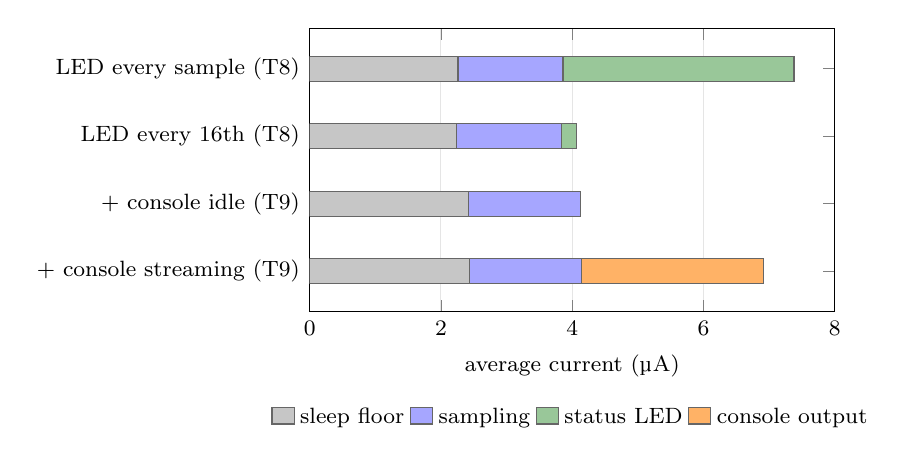
\begin{tikzpicture}
\begin{axis}[xbar stacked, scale only axis, width=0.55\textwidth, height=3.6cm, bar width=9pt,
  xmin=0, xmax=8, xlabel={average current (\textmu A)},
  ymin=0.4, ymax=4.6, ytick={1,2,3,4},
  yticklabels={{+ console streaming (T9)},{+ console idle (T9)},{LED every 16th (T8)},{LED every sample (T8)}},
  tick label style={font=\footnotesize}, label style={font=\footnotesize},
  legend style={font=\footnotesize, at={(0.5,-0.3)}, anchor=north, legend columns=4, draw=none},
  xmajorgrids, grid style={gray!20}]
\addplot[fill=gray!45, draw=black!60] coordinates {(2.26,4) (2.24,3) (2.42,2) (2.43,1)};
\addplot[fill=blue!35, draw=black!60] coordinates {(1.60,4) (1.60,3) (1.71,2) (1.71,1)};
\addplot[fill=green!45!black!40, draw=black!60] coordinates {(3.52,4) (0.22,3) (0,2) (0,1)};
\addplot[fill=orange!60, draw=black!60] coordinates {(0,4) (0,3) (0,2) (2.77,1)};
\legend{sleep floor, sampling, status LED, console output}
\end{axis}
\end{tikzpicture}
\caption{Average-current budget of the logger. Each pair of bars comes from one EnergyTrace session; the floors of the two sessions differ by $\sim$0.2\uA. The T9 build has no status LED.}
\label{fig:budget}
\end{figure}

% ---------------------------------------------------------------------
\testcase{T10}{Supercapacitor run, 82 minutes}{t:drain82}
  {Measure the real drain on the supercapacitor, and check the history log and the clock recovery on hardware.}
  {Debug configuration (-Ooff), all test switches 0.}
  {Supercap configuration.}
  {History records in order across every boot, each restored clock flagged and never behind an earlier record; a steady, linear discharge.}

\textbf{Procedure.}
\begin{enumerate}
  \item On USB, with J8 in Charge, start from an empty history (a fresh download clears it), then reset and power-cycle the board a few times to produce boot records.
  \item Set the clock with \code{time}.
  \item Move J8 to Use and unplug USB. Leave the board running.
  \item After 82 minutes, move J8 back to Charge, reconnect USB and dump the log with \code{hist}.
\end{enumerate}

\textbf{Results.} The log has 54 records (\code{data/e11\_hist.csv}). Moving J8 caused a power-on reset at 2954\,mV (record 11), and the board then logged on the supercapacitor for 82\,min, from 2961 to 2808\,mV (records 12--53), until USB was reconnected (record 54, power-on at 3296\,mV). Fig.~\ref{fig:drain} shows the discharge.

\begin{table}[H]
\centering\small
\begin{tabular}{@{}lccc@{}}
\toprule
Window & Records & Slope & Current at 0.22\,F \\
\midrule
First 10\,min & 6 & 46.7\,\textmu V/s & (10.3\uA, charge redistribution) \\
From 30\,min & 27 & 25.7\,\textmu V/s & 5.64\uA \\
Last 40\,min & 21 & 24.6\,\textmu V/s & 5.41\uA \\
\bottomrule
\end{tabular}
\end{table}

\begin{itemize}
  \item \textbf{Drain.} Over the first 10\,min the voltage fell faster than the load explains, as expected while charge redistributes in a freshly charged supercapacitor. After that the slope settled, with residuals within 2.6\,mV of a straight line. The total drain of 5.4--5.6\uA{} is 1--2\uA{} above the EnergyTrace measurements, which leave out the capacitor's leakage and the rest of its side of the board.
  \item \textbf{Running time.} At 24.6--25.7\,\textmu V/s the logger reaches the 2.2\,V cut-off 6.6--6.9\,h after the end of the run, or 8.2--8.6\,h after the 2.96\,V the charge reached. EnergyTrace alone, ignoring leakage, suggested 15--21\,h from 3.3\,V.
  \item \textbf{Temperature.} The die temperature fell by 2\,\textdegree C in the first 10\,min unplugged and then stayed flat, which is consistent with self-heating from the eZ-FET circuitry while USB is connected.
  \item \textbf{History and clock.} All nine boots were logged with their reason. Every boot after the first two restarted the clock from the newest logged time and flagged it as restored; sequence numbers and timestamps stayed in order. This includes the three reset-button boots: the RST pin causes a brown-out-level reset on this device and clears the RTC. After the final reconnect the clock restarted at 73\,078\,s, one second after the newest entry in the checkpoint's sample log, which had run two minutes past the last history record.
\end{itemize}

\begin{figure}[tbp]
\centering
\begin{tikzpicture}
\begin{groupplot}[group style={group size=1 by 2, vertical sep=3mm, x descriptions at=edge bottom},
  width=0.85\textwidth, xmin=0, xmax=82, enlarge x limits=false,
  tick label style={font=\footnotesize}, label style={font=\footnotesize},
  grid=major, grid style={gray!20}, xlabel={time on the supercapacitor (min)}]
\nextgroupplot[height=5.2cm, ylabel={VCC (mV)}, ymin=2790, ymax=2975]
  \addplot[only marks, mark=*, mark size=1.2pt, blue!70!black] table[x=tmin, y=vcc] {data/e11_drain.dat};
  \addplot[red!70!black, dashed, domain=30:82] {2808 + 24.6e-3*60*(82.0-x)};
\nextgroupplot[height=3cm, ylabel={temp. (\textdegree C)}, ymin=26.8, ymax=29.6, ytick={27,28,29}]
  \addplot[only marks, mark=*, mark size=1.2pt, orange!80!black] table[x=tmin, y=temp] {data/e11_drain.dat};
\end{groupplot}
\end{tikzpicture}
\caption{T10 supercapacitor run, one history record every 2\,min. The dashed line is the 24.6\,\textmu V/s fit over the last 40\,min, a 5.4\uA{} drain at 0.22\,F.}
\label{fig:drain}
\end{figure}

\textbf{Verdict:} \pass

% ---------------------------------------------------------------------
\testcase{T11}{Supercapacitor run, 12 minutes}{t:drain12}
  {Repeat the drain measurement on the release build before the overnight run, as a quick check.}
  {Release configuration (-O2), all test switches 0, freshly flashed.}
  {Supercap configuration.}
  {Drain within 20\,\% of T10; history records in order.}

\textbf{Procedure.} As T10, without setting the clock, for about 12 minutes.

\textbf{Results.} The log (\code{data/t11\_hist.csv}) starts with two reset-pin boots from flashing, then a power-on at 2787\,mV when J8 moved to Use (record 3). Seven 2-minute samples fell from 2796 to 2780\,mV, a slope of 21.7\,\textmu V/s with residuals under 1\,mV, or 4.8\uA. That is 12\,\% below T10. A lower voltage, the absence of redistribution after a fresh charge, and the optimized build may all contribute; this run cannot separate them. The temperature again fell by about 2\,\textdegree C.

One second before the final power-on, a sample read 2128\,mV and the logger entered deep sleep (record 11). The previous history record, 104\,s earlier, read 2780\,mV, and the supply was falling at only 1.3\,mV per minute. A real discharge cannot lose 650\,mV in 104\,s, so this was a dip in VCC while J8 was moved and USB reconnected. It did no harm here, but a single low reading should not be enough to enter deep sleep (issue I-1).

\textbf{Verdict:} \pass{} -- with issue I-1 logged.

% ---------------------------------------------------------------------
\testcase{T12}{Overnight supercapacitor run}{t:drainfull}
  {Run the complete scenario: logging from a full charge down to the 2.2\,V cut-off, the LPM3.5 hold with minute wakes, and the final brown-out, then read the history back.}
  {Release configuration (-O2), all test switches 0; the T11 build.}
  {Supercap configuration, J8 on Charge long enough for a full charge, clock set before unplugging.}
  {Deep-sleep entry within 50\,mV of 2.2\,V; minute wakes during the hold; history intact after the brown-out; logging time within 20\,\% of the T10 estimate.}

\textbf{Procedure.}
\begin{enumerate}
  \item On USB, with J8 in Charge, start from an empty history.
  \item Set the clock with \code{time} (record 1, 20:46:00).
  \item Move J8 to Use and unplug USB. Leave the board running overnight.
  \item The next morning, move J8 back to Charge, reconnect USB and dump the log with \code{hist}.
\end{enumerate}

\textbf{Results.} The log has 438 records (\code{data/t12\_hist.csv}): the clock setting, two power-on boots, 325 samples, one sleep record and 109 check-ins. Moving J8 caused a power-on at 2762\,mV (record 2). The board then logged for 10.8\,h, from 2775 to 2202\,mV, entered deep sleep, and held there for 1.8\,h until USB was reconnected (record 438, power-on at 3303\,mV). Fig.~\ref{fig:t12} shows the run.

\begin{table}[H]
\centering\small
\begin{tabular}{@{}llccc@{}}
\toprule
Phase & Clock time & VCC (mV) & Slope & Current at 0.22\,F \\
\midrule
Logging, first 3.5\,h & 20:47--00:17 & 2775 $\rightarrow$ 2555 & 17.1\,\textmu V/s & 3.8\uA \\
Logging, last 7.3\,h & 00:17--07:35 & 2555 $\rightarrow$ 2202 & 13.3\,\textmu V/s & 2.9\uA \\
Logging, whole phase & 20:47--07:35 & 2775 $\rightarrow$ 2202 & 14.7\,\textmu V/s & 3.2\uA \\
Deep sleep & 07:37--09:25 & 2196 $\rightarrow$ 2176 & 2.9\,\textmu V/s & 0.64\uA \\
\bottomrule
\end{tabular}
\end{table}

\begin{itemize}
  \item \textbf{Deep-sleep entry.} The last history sample read 2202\,mV at 07:35:33. A sample 82\,s later read 2199\,mV, and the logger saved and entered LPM3.5 (record 328). The readings had been approaching the threshold in 1--3\,mV steps for hours, so this was a real crossing of 2.2\,V, not the single bad reading of issue I-1.
  \item \textbf{Minute wakes.} All 109 check-ins are exactly 60\,s apart, from 07:37:00 to 09:25:00, with none missing. VCC never came back to the 2.6\,V resume level, so the logger stayed in deep sleep, as designed.
  \item \textbf{End of the run.} USB was reconnected at 09:25:01, one second after the last check-in. The clock was restored and every record is in order. The supply was still at 2.18\,V, far above brown-out, so the brown-out part of the scenario was not exercised. There was no spurious sleep record this time: the logger was already in deep sleep when the supply was disturbed.
  \item \textbf{Logging time.} The logger ran 10.8\,h from 2775\,mV down to 2.2\,V. A constant 5.4\uA, the T10 drain, predicts 6.5\,h for the same voltage range, so the real run lasted 67\,\% longer. The drain was not constant: it fell steadily from 4.3\uA{} to 2.7\uA{} (Fig.~\ref{fig:t12}c). The constant-drain running times derived from T10 and T11 are therefore pessimistic.
  \item \textbf{Why the drain falls.} In the first 3.5\,h the temperature held at about 27.7\,\textdegree C while the drain fell from 4.3 to 3.4\uA, so most of the fall comes with the voltage, and at the start partly with charge redistribution. A purely resistive leak would fall in proportion to the voltage, from 4.3 to about 3.5\uA{} between 2.74 and 2.24\,V; the measured fall to 2.7\uA{} is steeper. From 00:41 the room cooled from 27.7 to about 20\,\textdegree C, and supercapacitor leakage also falls with temperature. Voltage and temperature changed together after that, so this run cannot separate their effects.
  \item \textbf{Deep-sleep drain.} In deep sleep the supply fell by only 20\,mV in 1.8\,h, a drain of 0.64\uA{} with the capacitor's leakage included. That is well below the 2.10--2.25\uA{} EnergyTrace floor of T7, which covers only the board. Two effects may contribute: the supply here was about 2.19\,V, lower than in the EnergyTrace tests, and a supercapacitor's voltage recovers slowly after its load drops, which hides part of the drain. The 0.64\uA{} figure is best read as a lower bound. This adds to issue I-6.
  \item \textbf{Temperature.} After 03:00 the die temperature oscillates by about $\pm$0.5\,\textdegree C with a period of about 9.6\,min, consistent with a room air conditioner cycling on and off. The 2-minute sampling resolves it, and it does not show in VCC.
  \item \textbf{Charge level.} The run started at 2.76\,V, not from the full charge the setup asked for; T11 also started at 2.79\,V, while T10 reached 2.96\,V. The running time from a full charge was therefore not measured. Adding the 2.96 to 2.78\,V range at about 5\uA{} gives roughly 13\,h of logging from a 2.96\,V charge, an extrapolation.
\end{itemize}

\begin{figure}[tbp]
\centering
\begin{tikzpicture}
\begin{groupplot}[group style={group size=1 by 3, vertical sep=3mm, x descriptions at=edge bottom},
  width=0.85\textwidth, xmin=0, xmax=12.7, enlarge x limits=false, xtick={0,2,...,12},
  tick label style={font=\footnotesize}, label style={font=\footnotesize},
  grid=major, grid style={gray!20}, xlabel={time since J8 moved to Use (h); 0\,h is 20:46}]
\nextgroupplot[height=5.2cm, ylabel={VCC (mV)}, ymin=2150, ymax=2800]
  \addplot[only marks, mark=*, mark size=0.8pt, blue!70!black] table[x=th, y=vcc] {data/t12_drain.dat};
  \addplot[only marks, mark=*, mark size=0.8pt, orange!80!black] table[x=th, y=vcc] {data/t12_sleep.dat};
  \addplot[gray, dashed, domain=0:12.7] {2200};
  \node[font=\scriptsize, anchor=south west] at (axis cs:0.2,2200) {2.2\,V cut-off};
  \node[font=\scriptsize, anchor=north east, align=right] at (axis cs:12.5,2780) {(a) blue: logging, 2\,min samples\\orange: deep sleep, minute check-ins};
\nextgroupplot[height=3.4cm, ylabel={temp. (\textdegree C)}, ymin=19, ymax=30, ytick={20,25,30}]
  \addplot[only marks, mark=*, mark size=0.8pt, orange!80!black] table[x=th, y=temp] {data/t12_drain.dat};
  \node[font=\scriptsize, anchor=north east] at (axis cs:12.5,29.5) {(b)};
\nextgroupplot[height=4.6cm, ylabel={drain (\textmu A)}, ymin=0, ymax=5, ytick={0,1,...,5}]
  \addplot[blue!70!black, mark=*, mark size=1.3pt] table[x=th, y=iua] {data/t12_win.dat};
  \addplot[only marks, mark=triangle*, mark size=2.5pt, orange!80!black] coordinates {(11.75,0.64)};
  \node[font=\scriptsize, anchor=north east, align=right] at (axis cs:12.5,4.8) {(c) $C\,dV/dt$, 1\,h fits every 30\,min;\\triangle: whole deep-sleep phase};
\end{groupplot}
\end{tikzpicture}
\caption{T12 overnight supercapacitor run. (a) VCC, (b) die temperature during logging, (c) drain current derived from the slope of (a) at 0.22\,F.}
\label{fig:t12}
\end{figure}

\textbf{Verdict:} \pass{} -- with notes. Criteria 1 and 2 were met. Criterion 3 was not exercised, because the supply never reached brown-out. Criterion 4 was missed in the favourable direction: the logger ran 10.8\,h instead of the 6.5\,h a constant T10 drain predicts (+67\,\%), because the drain falls with the voltage. A repeat from a full charge down to brown-out is planned.

% =====================================================================
\section{Energy summary}

\begin{table}[H]
\centering\small
\caption{Average current and supercapacitor running time}
\label{tab:energy}
\begin{tabularx}{\textwidth}{@{}Lrr@{}}
\toprule
Firmware and method & Average & Running time \\
\midrule
Logger, LED every sample (T6, EnergyTrace) & 7.86\uA & 8.6\,h$^{a}$ \\
Final logger, idle console (T6, T8, T9, EnergyTrace) & 3.2--4.4\uA & 15--21\,h$^{a}$ \\
Deep-sleep hold below 2.2\,V (T7, EnergyTrace) & $\sim$2.2\uA & +8\,h$^{b}$ \\
\midrule
Final logger on the supercapacitor, $C\,dV/dt$ (T10) & 5.4\uA & 8.5\,h$^{c}$ \\
Final logger on the supercapacitor, $C\,dV/dt$ (T11) & 4.8\uA & 9.7\,h$^{c}$ \\
Final logger on the supercapacitor, 2.78 to 2.2\,V (T12) & 3.2\uA{} (4.3 to 2.7) & 10.8\,h$^{d}$ \\
Deep-sleep hold on the supercapacitor (T12) & 0.64\uA$^{e}$ & -- \\
\bottomrule
\multicolumn{3}{@{}l}{\footnotesize $^{a}$ $0.22 \times (3.3 - 2.2) = 0.242$\,C, leakage ignored.}\\
\multicolumn{3}{@{}l}{\footnotesize $^{b}$ $0.22 \times (2.2 - 1.9) = 0.066$\,C, down to the supply supervisor~\cite{ti_slase54}.}\\
\multicolumn{3}{@{}l}{\footnotesize $^{c}$ From 2.96 to 2.2\,V, the charge reached in T10; leakage included; constant drain assumed (pessimistic, see T12).}\\
\multicolumn{3}{@{}l}{\footnotesize $^{d}$ Measured, from 2.775\,V to the 2.2\,V cut-off.}\\
\multicolumn{3}{@{}l}{\footnotesize $^{e}$ Leakage included; a lower bound, see issue I-6.}
\end{tabularx}
\end{table}

The supercapacitor measurements are the ones to plan with: they include everything that drains the capacitor. T12 shows that this drain is not constant but falls with the voltage, so a running time is best measured, not extrapolated from one short run. EnergyTrace remains the right tool for comparing firmware variants, inside one capture.

% =====================================================================
\section{Issue log}
\label{sec:issues}

The issues below came from T7, T11, T12 and a review of the interrupt handling. None of them affected the test results in this report. All are open.

\begin{table}[H]
\centering\small
\caption{Open issues}
\label{tab:issues}
\begin{tabularx}{\textwidth}{@{}lLlL@{}}
\toprule
ID & Description & Found in & Impact and proposed fix \\
\midrule
I-1 & One reading below 2.2\,V sends the logger to deep sleep. A supply dip while moving J8 caused this in T11. & T11 & Up to a minute of lost logging per dip. Require two consecutive low readings (2\,s apart); a real discharge through 2.2\,V takes hours. \\
I-2 & \code{timer\_sleep\_ms} tests its done flag with interrupts enabled before entering LPM3. If the timer fires in between, the CPU sleeps until the next interrupt. & Review & Rare. A 2\,ms LED flash can last up to 2\,s (the next RTC tick), wasting energy and delaying a sample. Use the disable--check--sleep sequence the main loop already uses. \\
I-3 & The timer driver's status bytes are updated with read-modify-write outside critical sections, while its interrupt changes other bits of the same bytes. & Review & Latent; only one timer runs at a time today. Wrap the updates in critical sections. \\
I-4 & Sample requests coalesce while a console command runs. & Review & A full \code{hist} dump ($\sim$1.5\,min) skips about 45 samples. Interleave sampling with long dumps, or document it. \\
I-5 & The UART's blocking write and flush always return with interrupts enabled. & Review & Latent; they are only called with interrupts enabled. Restore the caller's interrupt state. \\
I-6 & The LPM3.5 floor (2.10--2.25\uA) is well above the datasheet value ($\sim$0.5\uA). On the supercapacitor, the whole deep-sleep drain, leakage included, was only 0.64\uA{} (T12), which contradicts that floor. & T7, T12 & Unexplained; the EnergyTrace offset, the higher supply in the EnergyTrace tests and voltage recovery in the supercapacitor are candidates. Measure with an independent microammeter, at a 2.2\,V supply, and with the J101 jumpers removed. \\
\bottomrule
\end{tabularx}
\end{table}

The review also confirmed what the interrupt handling does right: interrupt handlers only set flags or move single bytes, the main loop checks its flags and sleeps without a lost-wake-up race, shared variables are \code{volatile}, and each handler loops on its vector register until every pending flag is served.

% =====================================================================
\section{Conclusions}

\begin{itemize}
  \item \textbf{Power-loss safety.} The checkpoint store survived 36 random power cuts and a cut at every step of a save (T3, T4). The history log handled every simulated cut on the PC (T2) and every real boot on the board (T10, T11).
  \item \textbf{Power policy.} The deep-sleep cycle woke exactly on the RTC minute nine times out of nine and resumed with the clock continuous (T5).
  \item \textbf{Energy.} The final logger draws 3.2--4.4\uA{} by EnergyTrace (T6--T9). Limiting the status LED saved 45\,\%, and the idle console costs nothing measurable.
  \item \textbf{Real running time.} On the supercapacitor the drain is 4.8--5.4\uA{} near 2.8--2.96\,V (T10, T11), 1--2\uA{} above EnergyTrace because of the capacitor's own leakage. It falls with the voltage, to 2.7\uA{} near 2.2\,V, so the logger ran 10.8\,h from a 2.78\,V charge (T12), 67\,\% longer than a constant-drain estimate. Below 2.2\,V the deep-sleep hold drained only about 0.64\uA{} (T12).
  \item \textbf{Method.} EnergyTrace's absolute floor shifts by about 1\uA{} between sessions, so firmware variants must be compared inside one capture.
\end{itemize}

\textbf{Next steps.}
\begin{enumerate}
  \item Repeat T12 from a full charge (J8 on Charge until VCC stops rising) and let it run to brown-out, to complete criteria 3 and 4.
  \item Measure the drain against the voltage at a constant temperature, to separate the voltage and temperature effects seen in T12.
  \item Fix issues I-1 and I-2, then repeat T11.
  \item Measure the supercapacitor's leakage on its own, to separate it from the board's share of the 1--2\uA{} gap.
  \item Investigate I-6 with an independent microammeter.
  \item Add energy harvesting (for example a small solar cell) and adapt the sampling rate to the stored energy~\cite{colin2018capybara,hester2017future}.
\end{enumerate}

\bibliographystyle{IEEEtran}
\bibliography{references}

% =====================================================================
\appendix
\section{Module reference}
\label{app:modules}

\begin{table}[H]
\centering\small
\caption{Layer 1 drivers}
\begin{tabularx}{\textwidth}{@{}llL@{}}
\toprule
Driver & Responsibility & Key details \\
\midrule
hal\_common & Critical sections & \code{hal\_enter\_critical} / \code{hal\_exit\_critical} save and restore GIE \\
gpio & Ports P1--P8, PJ & Register-pointer table; PxSELC for 01$\leftrightarrow$10 function changes; driver owns PORT1--8 ISRs, loops on PxIV, callbacks return ``wake main'' \\
board & LaunchPad bring-up & Hold WDT $\rightarrow$ capture reset cause $\rightarrow$ all pins low $\rightarrow$ LEDs, buttons, UART idle, crystal pins $\rightarrow$ before-unlock hook $\rightarrow$ clear LOCKLPM5 $\rightarrow$ clear IFGs only if not an LPMx.5 wake; \code{board\_uart\_pins()} for the backchannel \\
cs & Clocks & DCO 1--16\,MHz with CS12 workaround and FRAM wait states (NWAITS\_1 above 8\,MHz); LFXT start with timeout, fallback to VLO; ms/\textmu s delays \\
pmm & Power and resets & Reset-cause bitmask from SYSRSTIV; boot reason; LPM0--4 entry from RAM; LPMx.5 entry; software BOR/POR \\
wdt & Watchdog & Watchdog and interval modes, kick, pause/resume; driver owns WDT\_VECTOR \\
\bottomrule
\end{tabularx}
\end{table}

\begin{table}[H]
\centering\small
\caption{Layer 2 and Layer 3 modules, and the history log}
\begin{tabularx}{\textwidth}{@{}llL@{}}
\toprule
Module & Responsibility & Key details \\
\midrule
ref & Internal reference & 1.2 / 2.0 / 2.5\,V; waits on GENBUSY, polls REFGENRDY; TLV calibration factors with sanity check \\
adc & VCC and die temperature & VCC via A31 (BATMAP) on the 2.0\,V reference, falling back to 1.2\,V below 2.4\,V; temperature via A30 (TCMAP) on 1.2\,V with TLV two-point calibration, averaged over 8 conversions; \SI{40}{\micro\second} sample time; ADC and REF off after each read \\
rtc & Calendar clock & Binary calendar mode; keeps time across LPM3.5 and non-brown-out resets; 125\,ms--2\,s periodic interrupt, minute/hour events, daily alarm; never clears interrupt flags during setup; \code{rtc\_to\_epoch}/\code{rtc\_from\_epoch} \\
timer & Timer\_A0--A4 on ACLK & Periodic, one-shot and sleep (LPM3) helpers; divider chosen automatically; up to 130\,s \\
crc & CRC16 hardware & CRC-16/CCITT-FALSE; self-test against a software reference (check value 0x29B1) \\
ckpt & Power-loss-safe store & Two FRAM slots (\code{\#pragma PERSISTENT}), 256-byte payload, commit order of Section~\ref{sec:ckpt}; newest valid slot restored \\
uart & eUSCI\_A0--A3, 8N1 & TX ring buffer fed by the TX interrupt; RX callback in interrupt context; baud registers from the user's-guide procedure; refuses $N<3$ \\
console & Command line & Echo, backspace, Ctrl-C; line parsed in the main loop into up to 6 words; input arriving while a line waits is refused with a bell; printing without \code{printf} \\
history & Long FRAM log & 1600 $\times$ 14-byte records; invalidate, fill, commit mark; 16-bit sequence; persistent hint repaired at boot \\
\bottomrule
\end{tabularx}
\end{table}

Red LED flashes at boot give the restart reason (1 power-on, 2 LPMx.5 wake, 3 reset pin, 4 watchdog, 5 software, 6 fault). Button S1 shows a supply gauge (one green flash per 100\,mV above 2.0\,V) and S2 erases the state.

\section{Files and data}

\begin{table}[H]
\centering\small
\begin{tabularx}{\textwidth}{@{}lL@{}}
\toprule
Path & Contents \\
\midrule
\code{drivers/} & hal\_common, gpio, board, cs, pmm, wdt, ref, adc, rtc, timer, crc, ckpt, uart \\
\code{app/} & Command console and history log \\
\code{main.c} & Logger, console commands and the test modes \\
\code{report/lab\_report.tex} & This report; \code{paper.tex} is the earlier paper-style version \\
\code{report/data/} & Plot data, and the \code{hist} dumps of T10 (\code{e11\_hist.csv}), T11 (\code{t11\_hist.csv}) and T12 (\code{t12\_hist.csv}) \\
\code{../dvt/*.csv} & EnergyTrace captures of T6--T9 \\
\bottomrule
\end{tabularx}
\end{table}

\section{T10 history log}

The full \code{hist} dump of T10. Records 1--9 are the boot tests on USB, record 10 the clock setting, 11--53 the run on the supercapacitor, and 54 the reconnect.

{\scriptsize\ttfamily
\begin{longtable}{@{}rrllllr@{}}
seq & t\_s & time & event & detail & vcc\_mv & temp\_c \\ \hline
\endhead
1 & 0 & 2026-01-01 00:00:00 & boot & reset pin & 3300 & \\
2 & 0 & 2026-01-01 00:00:00 & boot & reset pin & 3299 & \\
3 & 76 & 2026-01-01 00:01:16 & boot & power-on (clock restored) & 3297 & \\
4 & 115 & 2026-01-01 00:01:55 & sample & & 3301 & 29.5 \\
5 & 148 & 2026-01-01 00:02:28 & boot & reset pin (clock restored) & 3306 & \\
6 & 150 & 2026-01-01 00:02:30 & boot & reset pin (clock restored) & 3305 & \\
7 & 154 & 2026-01-01 00:02:34 & boot & power-on (clock restored) & 3312 & \\
8 & 178 & 2026-01-01 00:02:58 & boot & reset pin (clock restored) & 3306 & \\
9 & 227 & 2026-01-01 00:03:47 & sample & & 3306 & 29.4 \\
10 & 67920 & 2026-01-01 18:52:00 & clock & & & \\
11 & 67944 & 2026-01-01 18:52:24 & boot & power-on (clock restored) & 2954 & \\
12 & 68037 & 2026-01-01 18:53:57 & sample & & 2961 & 29.2 \\
13 & 68157 & 2026-01-01 18:55:57 & sample & & 2955 & 28.3 \\
14 & 68277 & 2026-01-01 18:57:57 & sample & & 2949 & 27.9 \\
15 & 68397 & 2026-01-01 18:59:57 & sample & & 2944 & 27.7 \\
16 & 68517 & 2026-01-01 19:01:57 & sample & & 2938 & 27.5 \\
\multicolumn{7}{@{}l}{\quad\textrm{\dots\ records 17--50: one sample every 2\,min, VCC falling steadily to 2817\,mV (Fig.~\ref{fig:drain}) \dots}} \\
51 & 72717 & 2026-01-01 20:11:57 & sample & & 2814 & 27.5 \\
52 & 72837 & 2026-01-01 20:13:57 & sample & & 2811 & 27.6 \\
53 & 72957 & 2026-01-01 20:15:57 & sample & & 2808 & 27.6 \\
54 & 73078 & 2026-01-01 20:17:58 & boot & power-on (clock restored) & 3296 & \\
\end{longtable}}

\end{document}
